\documentclass[11pt]{article}
\usepackage{times}
\usepackage{comment} % enables the use of multi-line comments (\ifx \fi)
\usepackage{fullpage} % changes the margin
\usepackage{graphicx}
\usepackage{subcaption}

\begin{document}
%Header-Make sure you update this information!!!!
\noindent
\large\textbf{Line W Analysis Update} \hfill \textbf{Jordan Thomas} \\
06/21/2017 \\

\section*{How can age and oxygen become decoupled?}

Age and oxygen are typically expected to be strongly negatively correlated in the
ocean interior (ventilated regions?). Under what conditions does this negative
relationshipbreak down, and even reverse?

Hypothesis is that age and oxygen become decoupled
when the flow is dominated by mixing as opposed to advection.


\section*{Results - Model Age-Oxygen Relationship:}
ESM2Mc model output along Line W suggests a region in the ocean interior where
this relationship is reversed (Figure 1). Positive correlation region lies on
neutral density surface $\gamma_{\mathrm{n}}$ = 27.0. To examine the structure
of this positive correlation region the age-oxygen correlation on
$\gamma_{\mathrm{n}}$ = 27.0 is shown in Figure 2.

On $\gamma_{\mathrm{n}}$ = 27.0, positive correlation region seen from Line W is
isolated from other positive correlation regions. Additionally, these waters are
to near the surface to be classified as Labrador Sea Water (27.83 $<$
$\gamma_{\mathrm{n}}$ $<$ 27.98).

\begin{figure*}[b!]
    \centering
    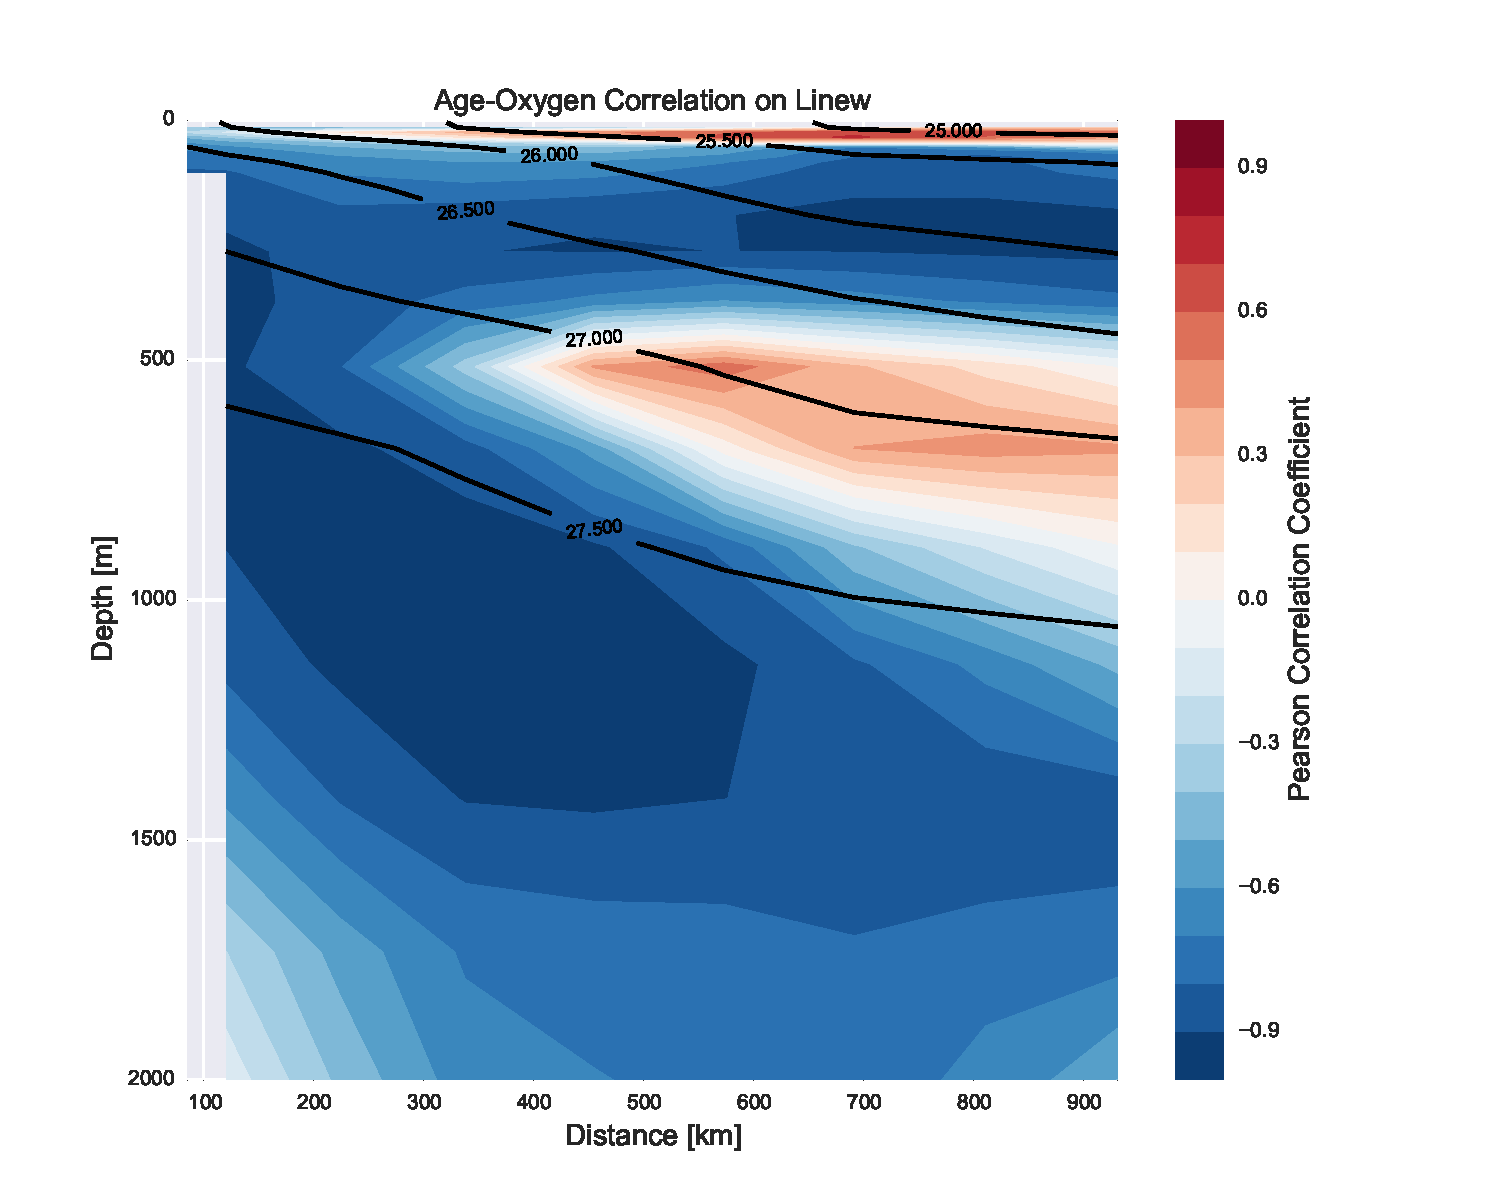
\includegraphics[height=3.7in]{correlation_on_linew.pdf}
    \caption{Pearson correlation coefficient for age vs oxygen interpolated to
    Line W.}
\end{figure*}

\clearpage

\begin{figure*}[t!]
    \centering
    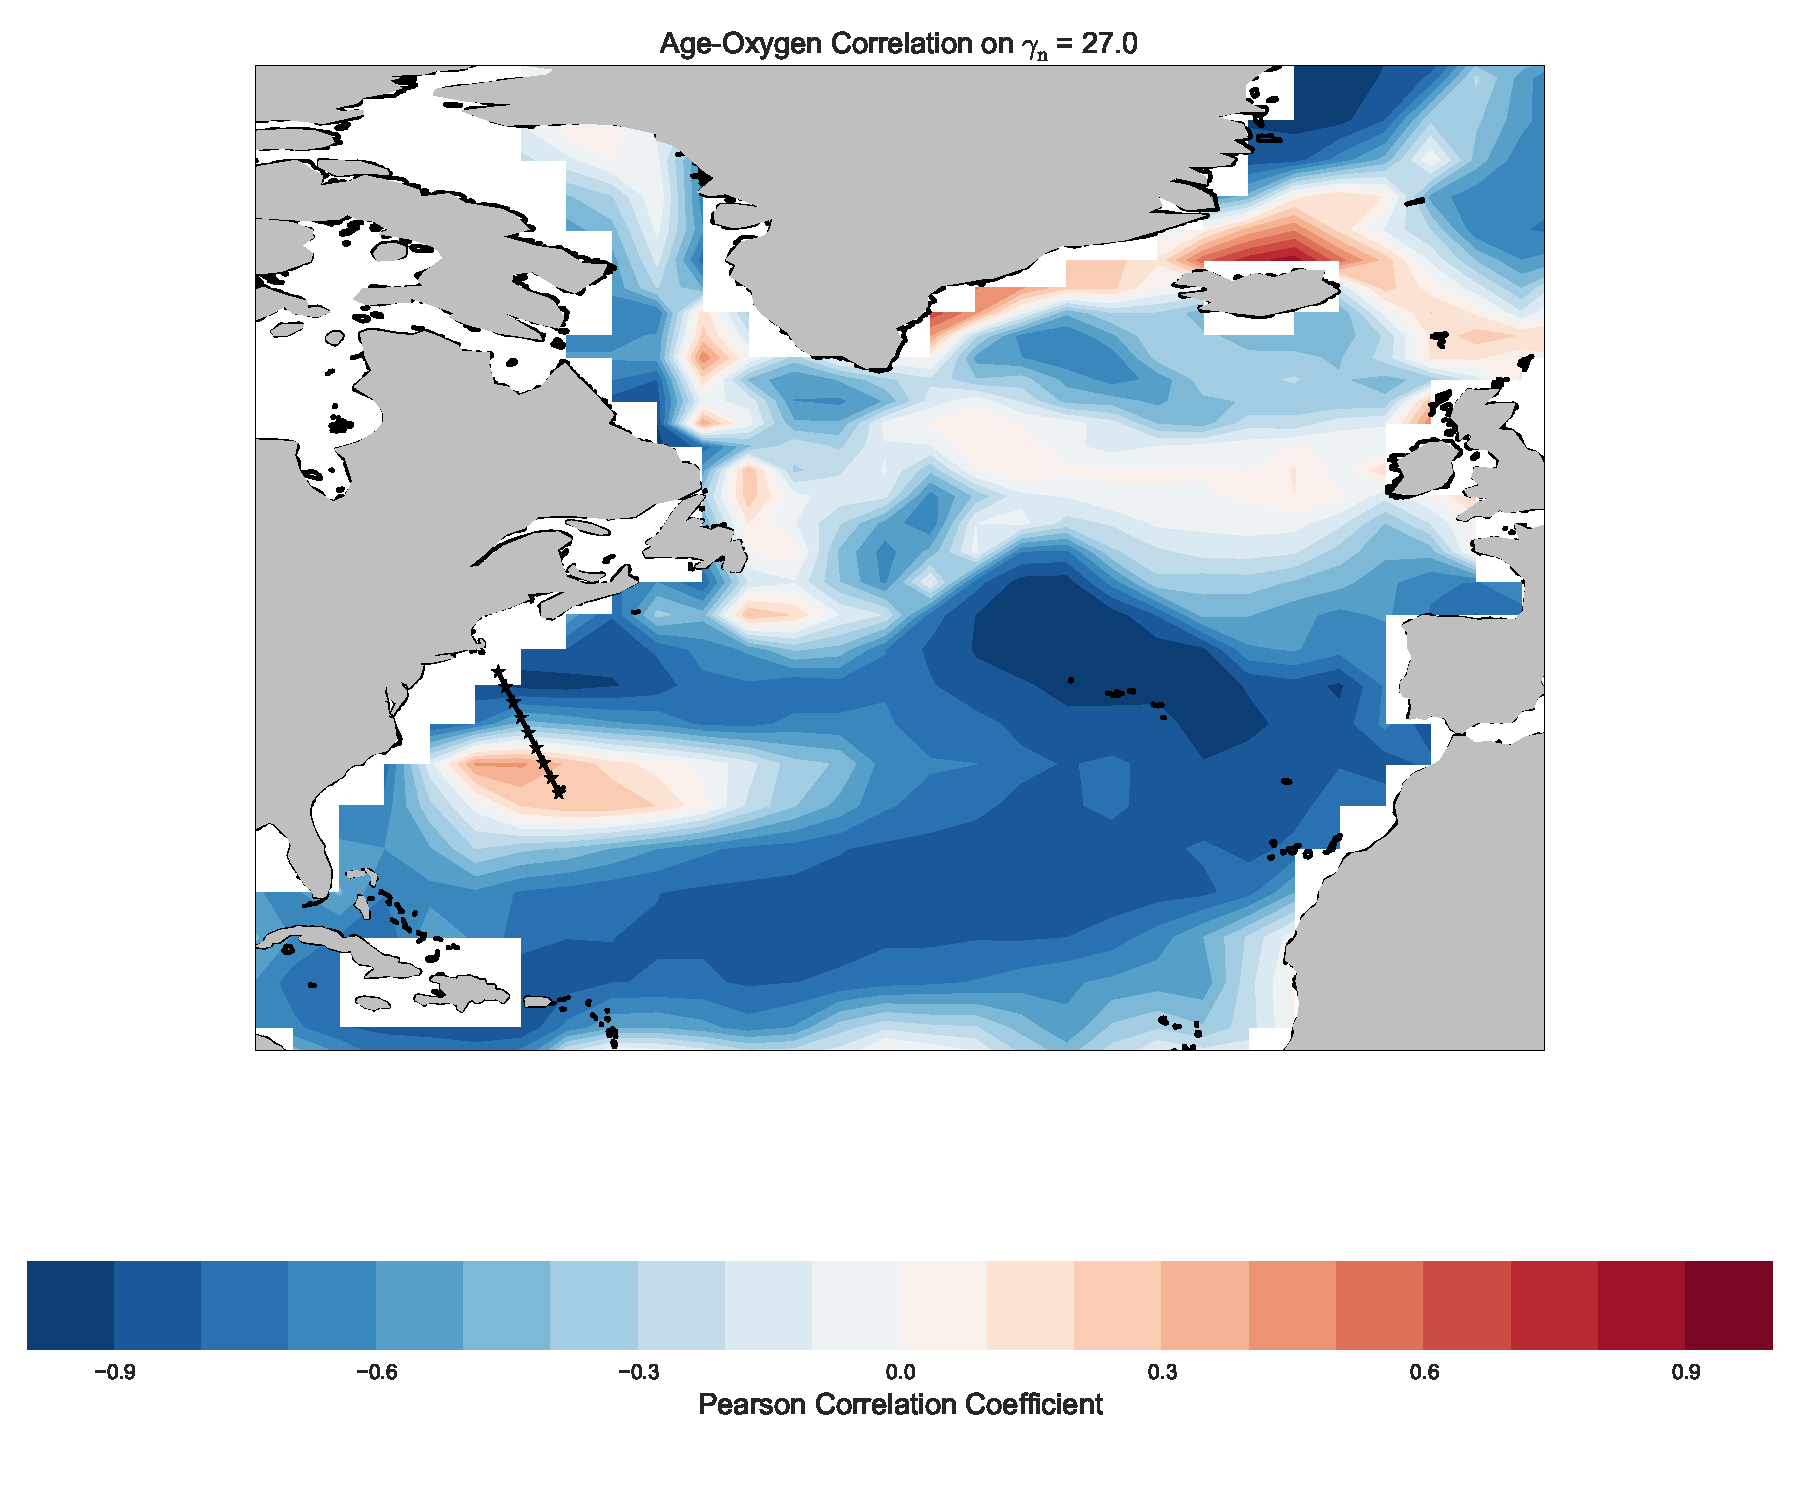
\includegraphics[height=3.5in]{correlation_on_27.pdf}
    \caption{Pearson correlation coefficient for age vs oxygen on neutral density
    surface 27.0.}
\end{figure*}

\begin{figure*}[b!]
    \centering
    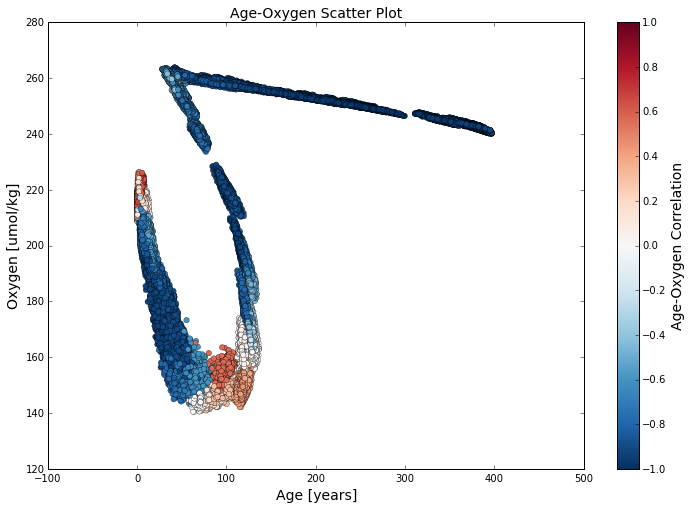
\includegraphics[height=3.5in]{Age-Oxygen_scatter.png}
    \caption{Scatter plot of age and oxygen averaged between distances 600-900 km.
    Colors indicate correlation coefficient. }
\end{figure*}

\section*{Results - Observations:}

Currently a little unsure about how observational data fits into age-oxygen
analysis. Figures 4 and 5 shows the age and oxygen observations along Line W.
Very few years extend observations past 300 km from Cape Cod making comparison
with model analysis difficult.

Using the two years from the NOAA proposal (Figure 6), we can look at the difference
between two relatively well-sampled years. The age-oxygen scatter plot for the two
years is shown in Figure 7 and shows that there is a slight difference in the surface
properties between the two years. Figure 8 shows the difference between these two
years for age and oxygen. There is a decrease (increase) in surface oxygen (age)
and the opposite signal directly below (around 500 dbs).

\section*{To-Do:}
Not really sure where to go from here. Would like to diagnose what causes
the positive correlation patch in the N. Atlantic interior. Possible analysis paths:
\begin{itemize}
  \item Calculate the local age and oxygen (vertical?) gradients.
  \item Analysis`upstream' (Labrador Sea?)
\end{itemize}

Would also like to figure out how to tie in the observational analysis. What
causes the significant increase in subsurface oxygen (with little change to
age) as seen in Figure 8. 



\begin{figure*}[b!]
    \centering
    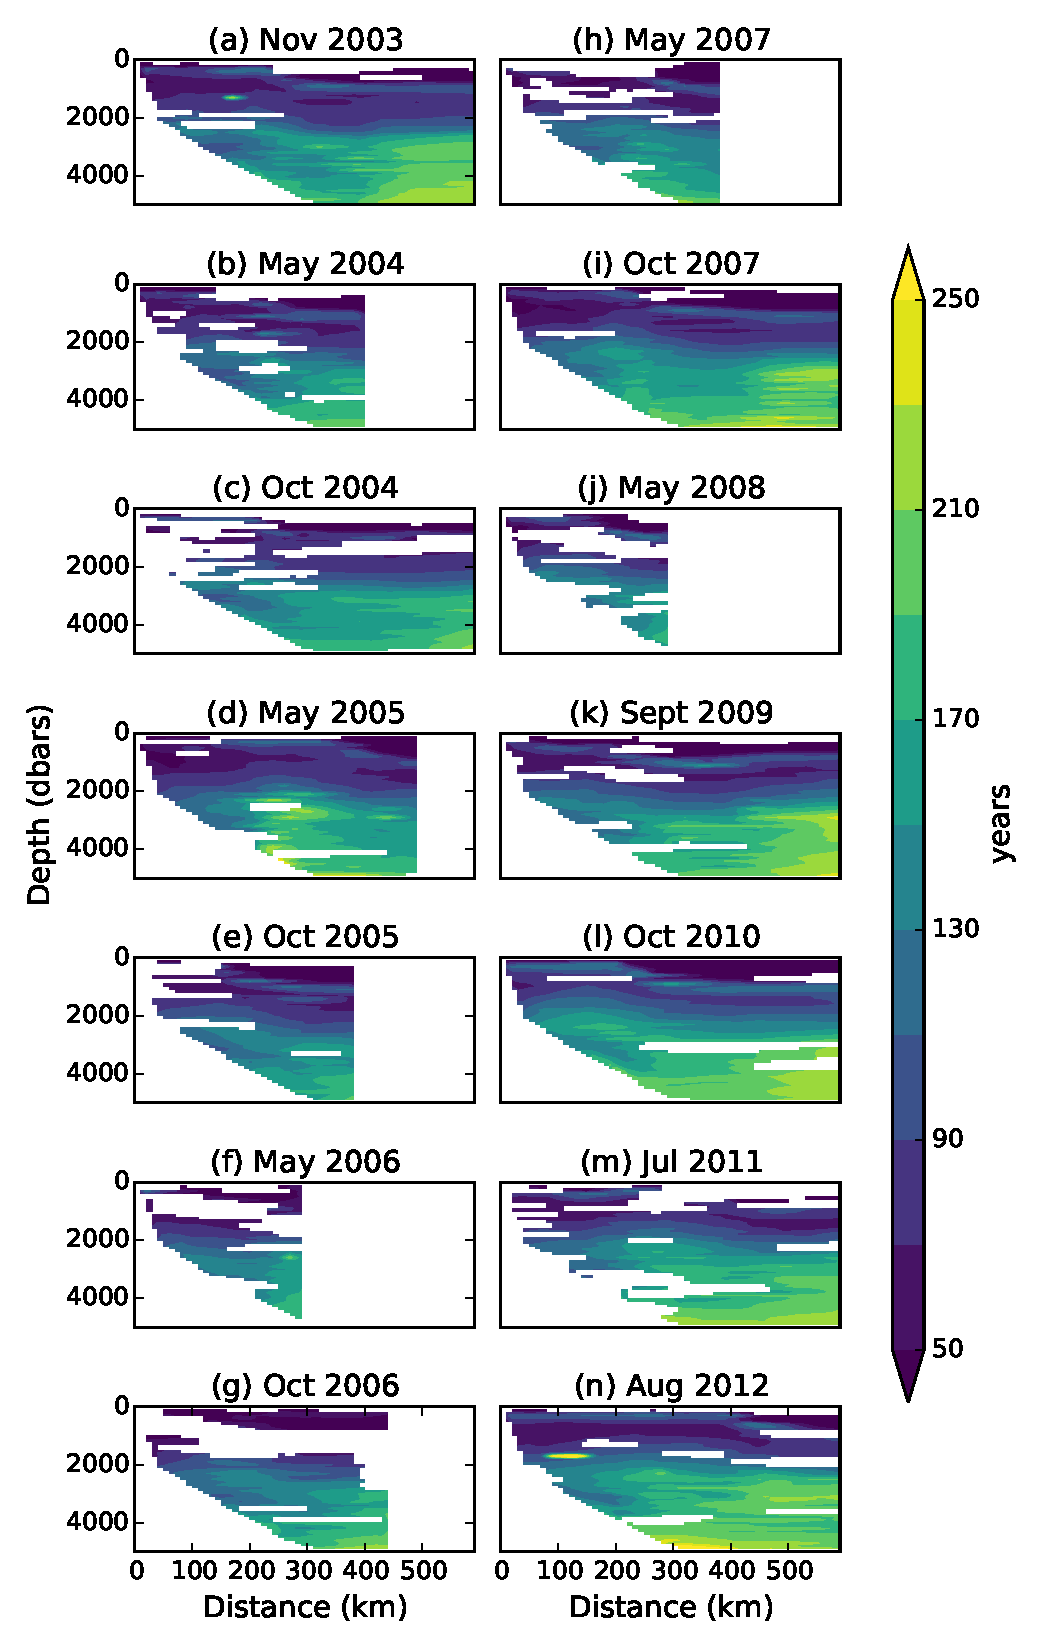
\includegraphics[height=8in]{linew_age_obs.pdf}
    \caption{Mean age observations along Line W. }
\end{figure*}

\begin{figure*}[b!]
    \centering
    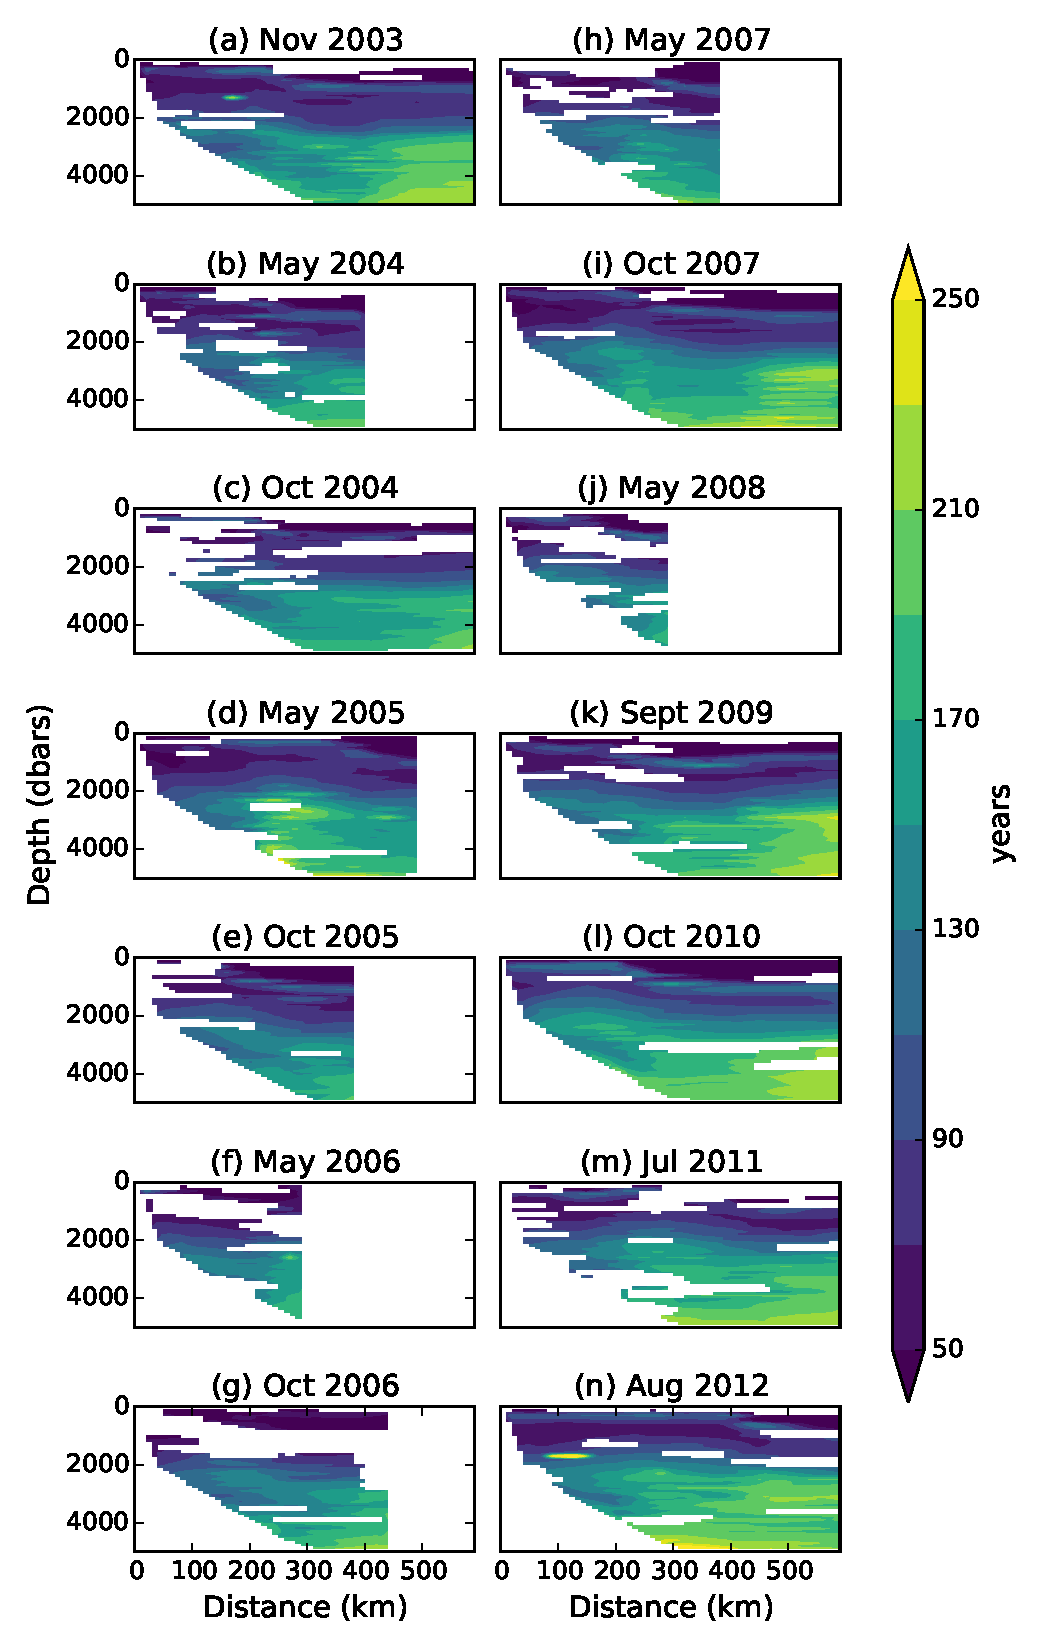
\includegraphics[height=8in]{linew_age_obs.pdf}
    \caption{Oxygen observations along Line W. }
\end{figure*}

\begin{figure*}[b!]
    \centering
    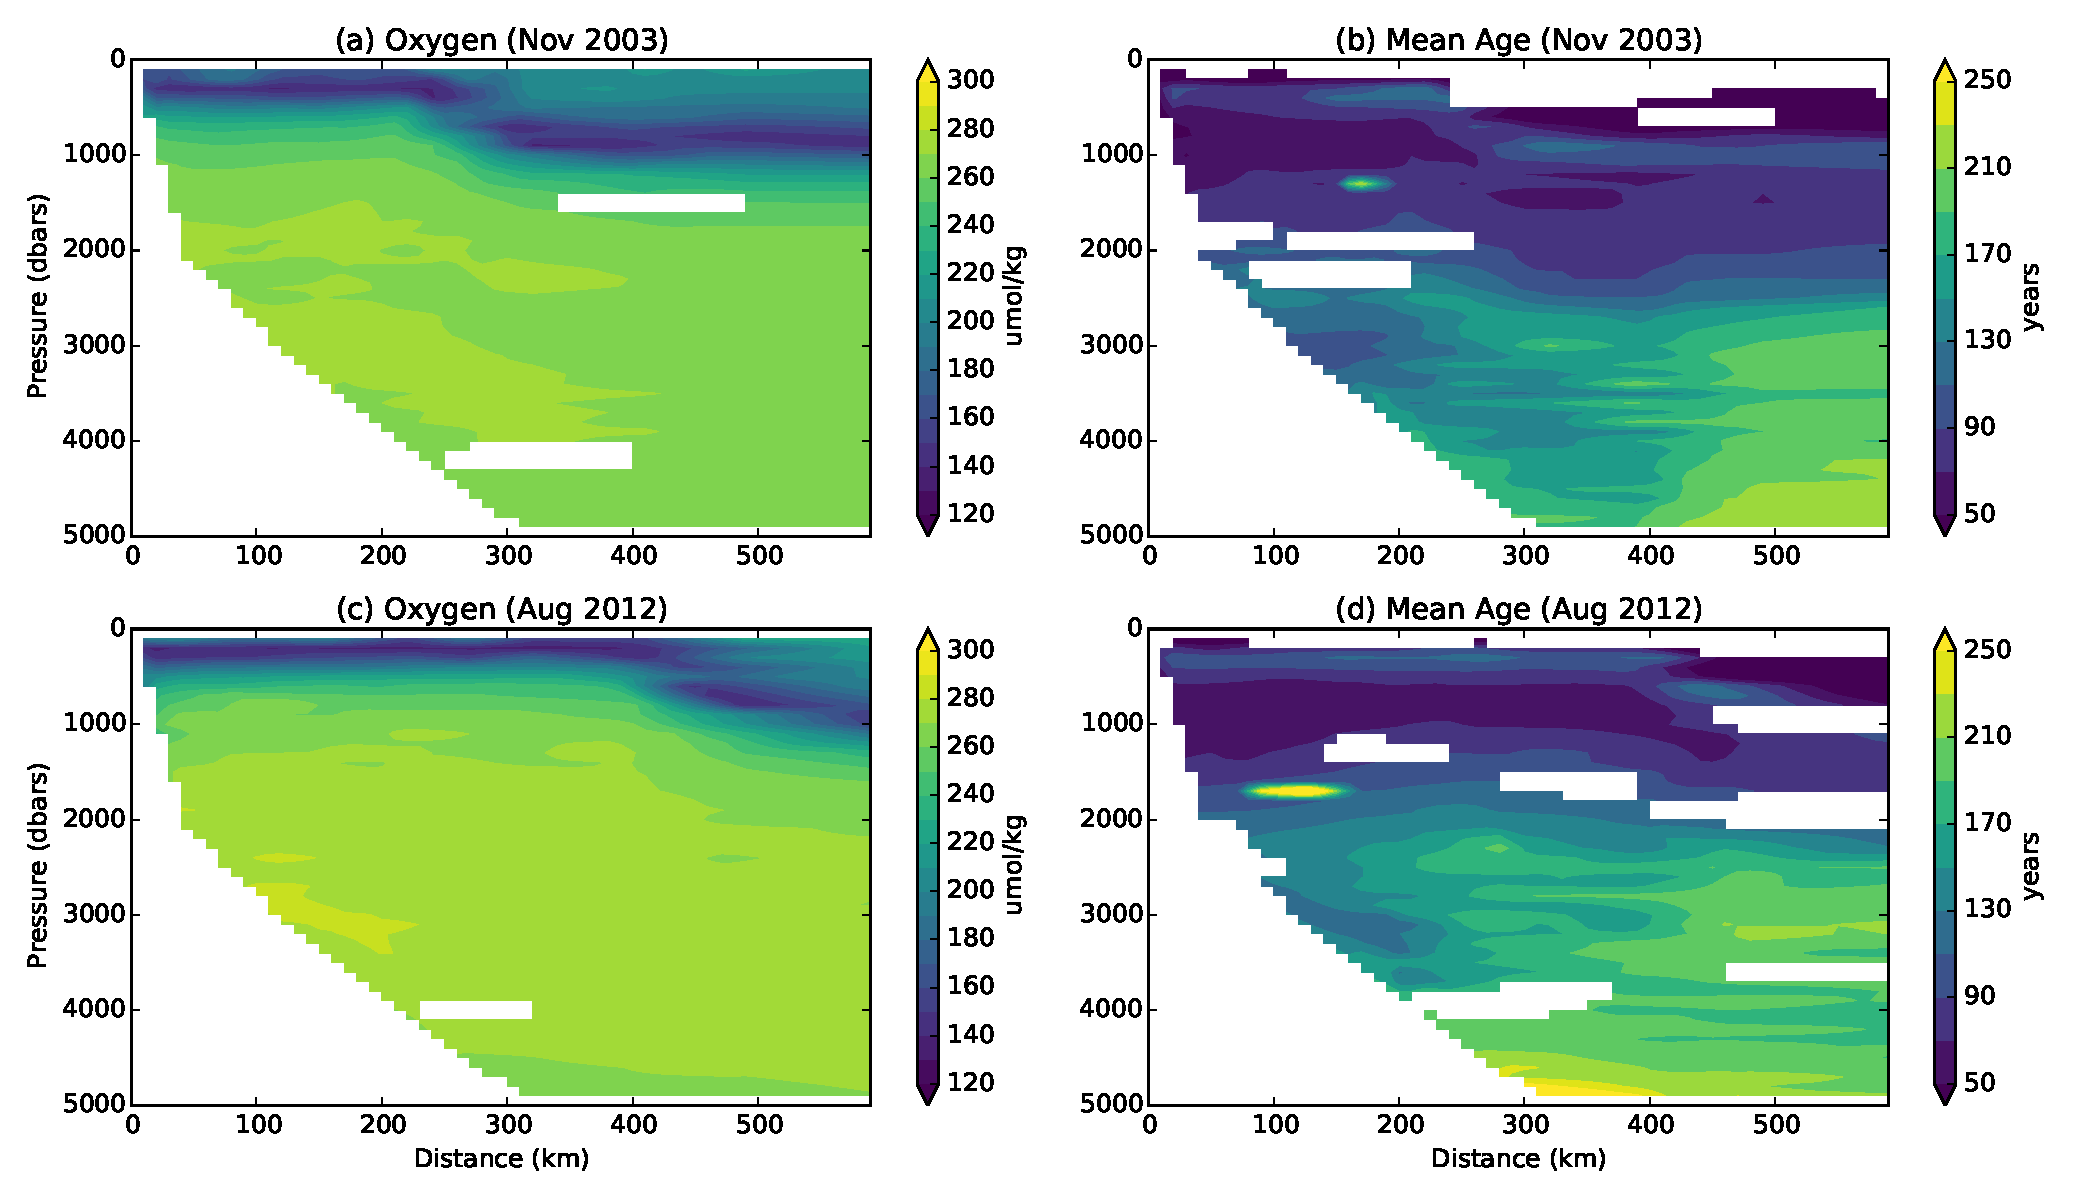
\includegraphics[height=4in]{age_oxygen_figure1.pdf}
    \caption{Age and oxygen observations along Line W for two years.}
\end{figure*}

\begin{figure*}[b!]
    \centering
    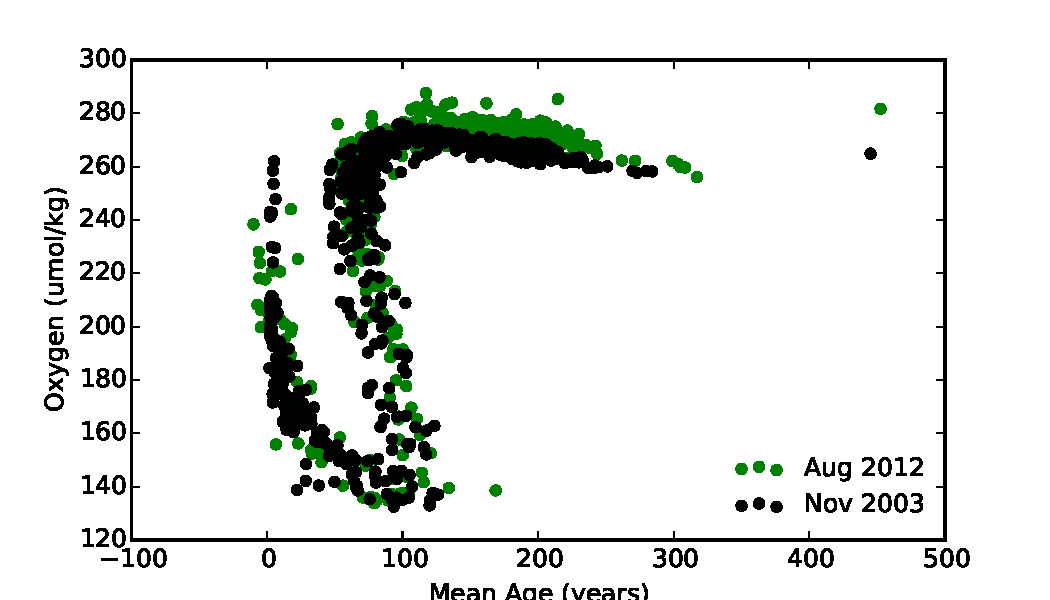
\includegraphics[height=3in]{age_oxygen_figure2.pdf}
    \caption{Age and oxygen scatter plot for both years}
\end{figure*}

\begin{figure*}[t!]
    \centering
    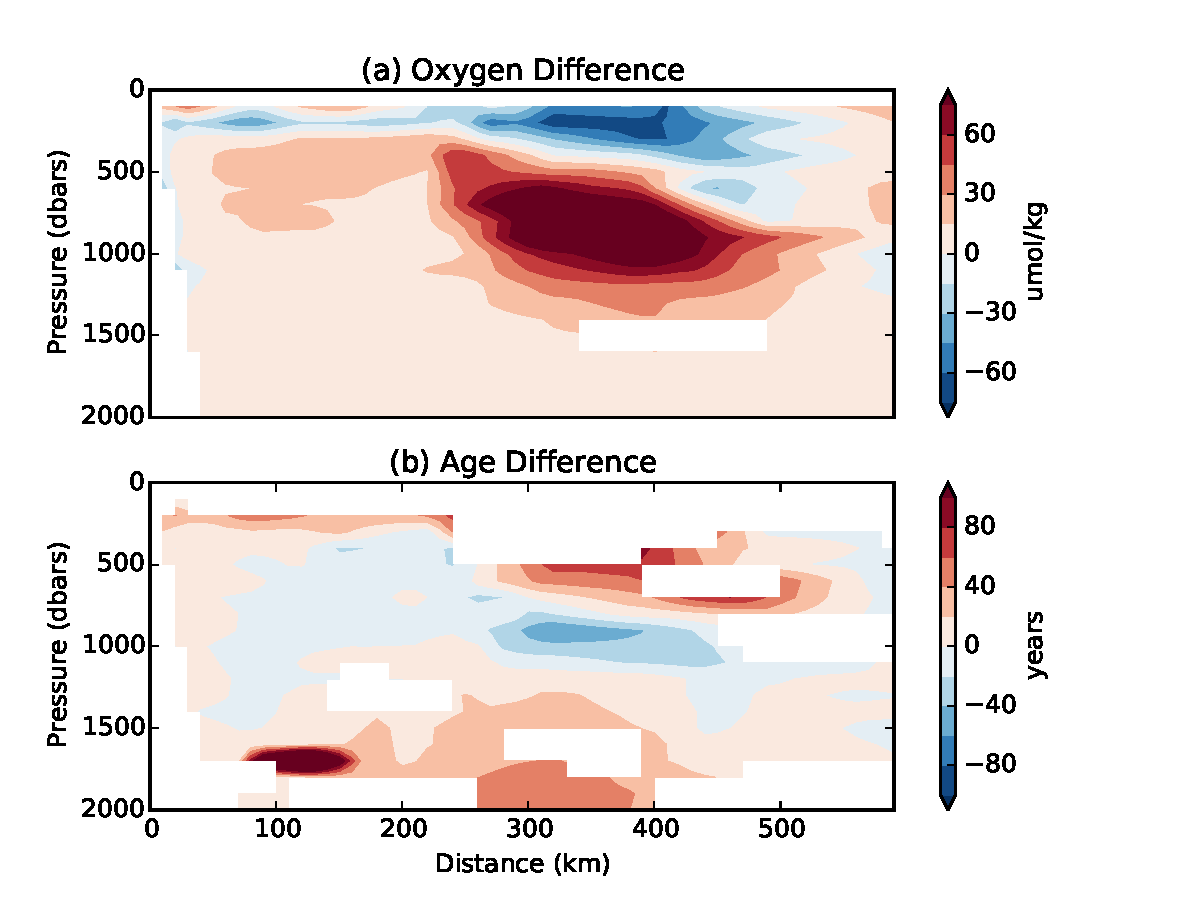
\includegraphics[height=4in]{age_oxygen_obs_difference.pdf}
    \caption{Aug 2012 - Nov 2003 difference for age and oxygen observations.}
\end{figure*}












\end{document}
